\documentclass[12pt,a4paper]{book}
\usepackage[utf8]{vietnam}
\usepackage{amsmath}
\usepackage{amsfonts}
\usepackage{xcolor}
\usepackage{titlesec}
\usepackage{mdframed}
\usepackage[unicode]{hyperref}
\usepackage{amssymb}
\usepackage{pgf,tikz,pgfplots}
\usepackage{hyperref}
\usepackage{draftwatermark}
\usepackage{graphicx}
\usepackage{cases} 
\pgfplotsset{compat=1.5}
\usepackage{mathrsfs}
\usetikzlibrary{arrows, calc}
\usepackage{float}
\usepackage{fancyhdr}
\pagestyle{headings}
\usepackage[left=2cm,right=2cm,top=2cm,bottom=2cm]{geometry}
\newmdenv[linecolor=black,skipabove=\topsep,skipbelow=\topsep,
leftmargin=-5pt,rightmargin=-5pt,
innerleftmargin=5pt,innerrightmargin=5pt]{mybox}
\newtheorem{theorem}{Định lí}[chapter]
\SetWatermarkAngle{60} %Góc là 60 độ

\SetWatermarkColor[gray]{0.8} %Màu xám, độ mờ là 80%

\SetWatermarkFontSize{5cm} %Độ dài của Watermark là 5cm

\SetWatermarkScale{0.1} %Độ phóng to

\SetWatermarkText{Tổng hợp bởi Nguyễn Văn Lộc} %Nội dung Watermark

\begin{document}
\begin{titlepage}
\begin{center}
\textbf{ĐẠI HỌC QUỐC GIA THÀNH PHỐ HỒ CHÍ MINH}\\
\textbf{TRƯỜNG ĐẠI HỌC KHOA HỌC TỰ NHIÊN}
\end{center}
\vspace{4 cm}
\begin{center}
\fontsize{20}{16}\selectfont
\centerline{\textbf{ĐẠI SỐ TUYẾN TÍNH}}
\end{center}

\vspace{14 cm}
\centerline{\textbf{\textit{Tổng hợp bởi Nguyễn Văn Lộc}}}
\end{titlepage}
\tableofcontents
\newpage
\documentclass[12pt,a4paper]{article}
\usepackage[utf8]{vietnam}
\usepackage{amsmath}
\usepackage{amsfonts}
\usepackage{xcolor}
\usepackage{titlesec}
\usepackage{mdframed}
\usepackage{amssymb}
\usepackage{graphicx}
\usepackage{cases} 
\usepackage{pgfplots}
\pgfplotsset{compat=1.5}
\usepackage{mathrsfs}
\usetikzlibrary{arrows}
\usepackage{fancyhdr}
\usepackage{float}
\usepackage{enumerate}
\usepackage{enumitem}
\pagestyle{fancy}
\pagestyle{empty}
\usepackage[left=2cm,right=2cm,top=2cm,bottom=2cm]{geometry}
\author{Nguyễn Văn Lộc}
\newmdenv[linecolor=black,skipabove=\topsep,skipbelow=\topsep,
leftmargin=-5pt,rightmargin=-5pt,
innerleftmargin=5pt,innerrightmargin=5pt]{mybox}
\begin{document}
\fancyhf{}
\lhead{}
\chead{}
\rhead{}
\cfoot{}
\rfoot{\thepage}
\lfoot{}
\pagestyle{fancy}
\renewcommand{\headrulewidth}{0pt}
\renewcommand{\footrulewidth}{0pt}
\begin{mybox}
\textbf{Họ và tên:} Nguyễn Văn Lộc\\
\textbf{MSSV:} 20120131\\
\textbf{Lớp:} 20CTT1
\end{mybox}
\begin{center}
\fontsize{16}{14}\selectfont
\textbf{Bài tập môn Xác suất thống kê}\\
\textbf{Chương 1: Đại cương về xác suất}
\end{center}
Các bài tập được làm: 1, 2, 3, 4, 6, 7, 8, 9, 10, 11, 13\\
\textbf{Bài 1.} \textit{Một thí sinh đi thi chỉ thuộc $18$ câu trong tổng số $25$ câu hỏi. Đề thi có $3$ câu hỏi. Tính xác suất thí sinh này:}
\begin{enumerate}[label=(\alph*)]
\item \textit{trả lời được $3$ câu.}\\
Không gian mẫu: $n_{\Omega} = C^3_{25}.$\\
Gọi $A$ là biến cố: "thí sinh này trả lời được $3$ câu."\\
Số cách lấy ra $3$ câu hỏi mà thí sinh này thuộc hết là: $n_A = C^3_{18}.$
$$\Rightarrow P\left( A \right) = \frac{{{n_A}}}{{{n_\Omega }}} = \frac{{C_{18}^3}}{{C_{25}^3}} = \frac{{204}}{{575}}.$$
\item \textit{trả lời được ít nhất $2$ câu.}\\
Gọi $B$ là biến cố: "thí sinh này trả lời được ít nhất $2$ câu."\\
Trường hợp 1: thí sinh này trả lời được đúng $2$ câu.\\
Số cách lấy ra $3$ câu hỏi mà thí sinh này trả lời được đúng $2$ câu là: $C^2_{18} C^1_{7}.$\\
Trường hợp 2: thí sinh này trả lời được cả $3$ câu.\\
Số cách lấy ra $3$ câu hỏi mà thí sinh này trả lời được hết hết là: $C^3_{18}.$\\
$$\Rightarrow n_B = C^2_{18} C^1_{7} + C^3_{18}.$$
$$ \Rightarrow P\left( B \right) = \frac{{{n_B}}}{{{n_\Omega }}} = \frac{{C_{18}^2C_7^1 + C_{18}^3}}{{C_{25}^3}} = \frac{{1887}}{{2300}}.$$
\end{enumerate}
\textbf{Bài 2.} \textit{Có hai lô sản phẩm. Lô thứ nhất có $10$ sản phẩm loại I và $2$ sản phẩm loại II; lô thứ hai có $16$ sản phẩm loại I và $4$ sản phẩm loại II. Từ mỗi lô lấy ngẫu nhiên $1$ sản phẩm, sau đó từ $2$ sản phẩm đã lấy ra lấy ngẫu nhiên $1$ sản phẩm. Tính xác suất sản phẩm lấy ra cuối cùng là loại I.}\\
Không gian mẫu: ${n_\Omega } = C_{12}^1C_{20}^1C_2^1 = 480.$\\
Gọi $A$ là biến cố: "sản phẩm lấy ra cuối cùng là loại I."\\
Trường hợp 1: cả hai sản phẩm lấy ra từ hai lô đều là loại I.\\
Số cách lấy ra thỏa mãn biến cố $A$ là: $C^1_{10} C^1_{16} C^1_{2}.$\\
Trường hợp 2: sản phẩm lấy ra từ lô thứ nhất là loại I, sản phẩm lấy ra từ lô thứ hai là loại II.\\
Số cách lấy ra thỏa mãn biến cố $A$ là: $C^1_{10} C^1_{4} C^1_{1}.$\\
Trường hợp 3: sản phẩm lấy ra từ lô thứ nhất là loại II, sản phẩm lấy ra từ lô thứ hai là loại I.\\
Số cách lấy ra thỏa mãn biến cố $A$ là: $C^1_2 C^1_{16} C^1_1.$\\
Vậy tổng số cách lấy ra thỏa mãn biến cố $A$ là: 
$${n_A} = C_{10}^1C_{16}^1C_2^1 + C_{10}^1C_4^1C_1^1 + C_2^1C_{16}^1C_1^1 = 392.$$
$$ \Rightarrow P\left( A \right) = \frac{{{n_A}}}{{{n_\Omega }}} = \frac{{392}}{{480}} = \frac{{49}}{{60}}.$$
\textbf{Bài 3.} \textit{Một người có ba chỗ ưa thích như nhau để câu cá, xác suất câu được cá ở những chỗ đó lần lượt là $0.6, 0.7, 0.8.$ Người đó vào chỗ thả câu $3$ lần và chỉ câu được $1$ con cá. Tính xác suất con cá câu được ở chỗ thứ nhất.}\\
Gọi $A_i$ là biến cố: "người đó đi câu ở chỗ thứ $i,$ $i = 1, 2, 3$ Ta được: $P \left( {A_i} \right) = \frac{1}{3},$ $i = 1, 2, 3.$\\
Gọi $B$ là biến cố: "câu được $1$ con cá trong $3$ lần đi câu tại địa điểm đã chọn."\\
Ta thấy đâu là mô hình các phép thử tuân theo lược đồ Bernoulli. Do đó, áp dụng công thức Bernoulli, ta được:
$$P\left( {\left. B \right|{A_1}} \right) = C_3^1{\left( {0.6} \right)^1}{\left( {0.4} \right)^2} = \frac{{36}}{{125}}.$$
$$P\left( {\left. B \right|{A_2}} \right) = C_3^1{\left( {0.7} \right)^1}{\left( {0.3} \right)^2} = \frac{{189}}{{1000}}.$$
$$P\left( {\left. B \right|{A_3}} \right) = C_3^1{\left( {0.8} \right)^1}{\left( {0.2} \right)^2} = \frac{{12}}{{125}}.$$
$$ \Rightarrow P\left( B \right) = \sum\limits_{i = 1}^3 {P\left( {{A_i}} \right)} P\left( {\left. B \right|{A_i}} \right) = \frac{1}{3}\left( {\frac{{36}}{{125}} + \frac{{189}}{{1000}} + \frac{{12}}{{125}}} \right) = \frac{{191}}{{1000}}.$$
Áp dụng công thức Bayes, ta được:
$$P\left( {\left. {{A_1}} \right|B} \right) = \frac{{P\left( {{A_1}} \right)P\left( {\left. B \right|{A_1}} \right)}}{{P\left( B \right)}} = \frac{{96}}{{191}}.$$
\textbf{Bài 4.} \textit{Trên đoạn thẳng $OA$ ta gieo một cách ngẫu nhiên hai điểm $B, C$ có tọa độ tương ứng là $OB = x, OC = y$ $\left( {y \geqslant x} \right).$ Tìm xác suất sao cho độ dài đoạn $BC$ bé hơn độ dài đoạn $OB.$}\\
\begin{figure}[H]
\begin{center}
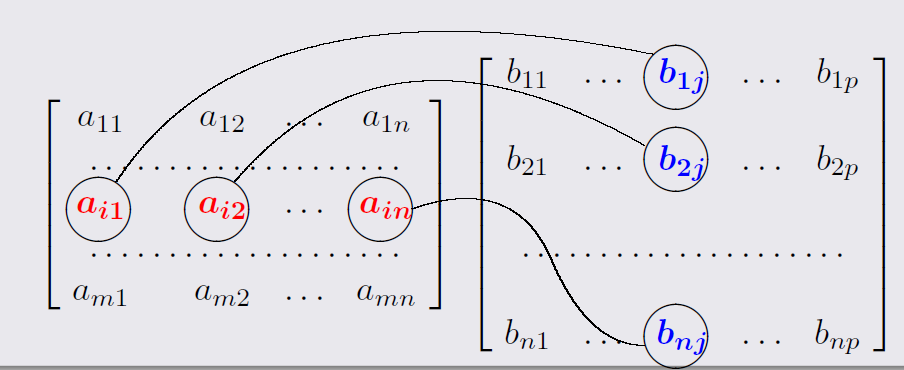
\includegraphics[scale=1]{C1_1}
\end{center}
\end{figure}
Gọi $A$ là biến cố: "độ dài đoạn $BC$ bé hơn độ dài đoạn $OB$".\\
Gọi độ dài đoạn $OA$ là $l.$\\
Độ dài đoạn $BC$ là $BC = y - x.$\\
Độ dài đoạn $BC$ bé hơn độ dài đoạn $OB$ có nghĩa là $y - x < x \Leftrightarrow y < 2x.$\\
Vậy, $y$ thỏa mãn $x \leqslant y < 2x.$
\begin{figure}[H]
\begin{center}
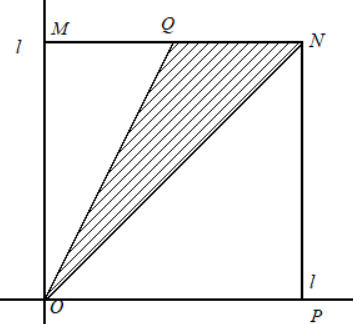
\includegraphics[scale=0.8]{C1_2}
\end{center}
\end{figure}
Miền thỏa mãn đề bài là tam giác $ONQ.$
$$ \Rightarrow P\left( A \right) = \frac{{{S_{ONQ}}}}{{{S_{OMN}}}} = \frac{1}{2}.$$
\textbf{Bài 6.} \textit{Một chuỗi cửa hàng sơn kinh doanh sơn mủ và sơn bán bóng. Dựa trên doanh số bán hàng trong thời gian dài, xác suất để một khách hàng sẽ mua sơn mủ là $0.75.$ Trong số những người mua sơn mủ, $60\%$ cũng mua con lăn. Nhưng chỉ $30\%$ người mua sơn bán bóng mua con lăn. Một người mua được chọn ngẫu nhiên mua một con lăn và một hộp sơn. Tính xác suất hộp sơn đó là sơn mủ.}\\
Gọi $A$ là biến cố: "Người mua đó mua sơn mủ."\\
$B$ là biến cố: "Người mua đó mua sơn bán bóng."\\
$C$ là biến cố: "Người mua đó mua con lăn."\\
Theo đề bài, ta có:
$$P \left( A \right) = 0.75 \Rightarrow P \left( B \right) = 0.25.$$
$$P \left( {\left. C \right|A} \right) = 0.6.$$
$$P \left( {\left. C \right|B} \right) = 0.3.$$
Áp dụng công thức xác suất toàn phần, ta được:
$$P\left( C \right) = P\left( A \right)P\left( {\left. C \right|A} \right) + P\left( B \right)P\left( {\left. C \right|B} \right) = 0.75 \cdot 0.6 + 0.25 \cdot 0.3 = \frac{{21}}{{40}}.$$
Áp dụng công thức Bayes, ta được: 
$$P\left( {\left. A \right|C} \right) = \frac{{P\left( A \right)P\left( {\left. C \right|A} \right)}}{{P\left( C \right)}} = \frac{{0.75 \cdot 0.6}}{{\frac{{21}}{{40}}}} = \frac{6}{7}.$$
\textbf{Bài 7.} \textit{Giả sử khảo sát tình trạng hư hỏng của các điện thoại tại một trung tâm bảo hành điện thoại, người ta nhận thấy $90\%$ số điện thoại bị lỗi phần mềm, $30\%$ số điện thoại bị lỗi phần cứng và tất cả điện thoại ở trung tâm bảo hành này đều bị ít nhất một trong hai lỗi trên. Tính xác suất để một điện thoại bảo hành ở trung tâm này chỉ bị lỗi phần mềm.}\\
Gọi $x$ là số điện thoại tại trung tâm bảo hành.\\
Gọi $A_1$ là số điện thoại bị lỗi phần cứng, $A_2$ là số điện thoại bị lỗi phần mềm.\\
Theo đề bài, ta có:
$$\left\{ \begin{gathered}
  \left| {{A_1}} \right| = 0.9x \hfill \\
  \left| {{A_2}} \right| = 0.3x \hfill \\
  \left| {{A_1} \cup {A_2}} \right| = x \hfill \\ 
\end{gathered}  \right.$$
Theo nguyên lý bù trừ, ta được $\left| A_1 \cap A_2 \right| = 0.2x.$\\
Vậy số điện thoại chỉ bị lỗi phần mềm là $0.7x,$ nghĩa là xác suất điện thoại chỉ bị lỗi phần mềm là $0.7.$\\
\textbf{Bài 8.} \textit{Một dây chuyền lắp ráp nhận các chi tiết từ hai nhà máy khác nhau. Tỉ lệ chi tiết do nhà máy thứ nhất cung cấp là $60\%,$ của nhà máy thứ hai là $40\%.$ Tỉ lệ chính phẩm của nhà máy thứ nhất là $90\%$, của nhà máy thứ hai là $85\%.$ Lấy ngẫu nhiên một chi tiết trên dây chuyền và thấy rằng nó tốt. Tìm xác suất để chi tiết đó do nhà máy thứ nhất sản xuất.} \\
Gọi $A_i$ là biến cố: "chi tiết đó được sản xuất ở nhà máy thứ $i$, $i = 1, 2$."\\
Gọi $B$ là biến cố: "chi tiết đó là chi tiết tốt".\\
$$P\left( {{A_1}} \right) = 0.6,P\left( {{A_2}} \right) = 0.4$$
$$P\left( {\left. B \right|{A_1}} \right) = 0.9$$
$$P\left( {\left. B \right|{A_2}} \right) = 0.85$$
Áp dụng công thức xác suất toàn phần:
$$ \Rightarrow P\left( B \right) = P\left( {{A_1}} \right)P\left( {\left. B \right|{A_1}} \right) + P\left( {{A_2}} \right)P\left( {\left. B \right|{A_2}} \right) = 0.88.$$
Áp dụng công thức Bayes:
$$P\left( {\left. {{A_1}} \right|B} \right) = \frac{{P\left( {{A_1}} \right)P\left( {\left. B \right|{A_1}} \right)}}{{P\left( B \right)}} = \frac{{27}}{{44}}.$$
\textbf{Bài 9.} \textit{Một nhà máy có ba phân xưởng $A, B, C$ tương ứng làm ra $25\%, 35\%, 40\%$ tổng sản phẩm của nhà máy. Giả sử xác suất làm ra một sản phẩm hỏng của các phân xưởng là $0.01, 0.02, 0.025.$ Hãy tính xác suất nhận được một sản phẩm hỏng.}\\
Gọi $A_1, A_2, A_3$ lần lượt là các biến cố: "sản phẩm đó sản xuất tại phân xưởng $A,$" "sản phẩm đó sản xuất tại phân xưởng $B,$" "sản phẩm đó sản xuất tại phân xưởng $C.$"\\
Gọi $B$ là biến cố: "sản phẩm đó là sản phẩm hỏng."\\
$$\left\{ \begin{gathered}
  P\left( {{A_1}} \right) = 0.25 \hfill \\
  P\left( {{A_2}} \right) = 0.35 \hfill \\
  P\left( {{A_3}} \right) = 0.4 \hfill \\ 
\end{gathered}  \right.$$
$$\left\{ \begin{gathered}
  P\left( {\left. B \right|{A_1}} \right) = 0.01 \hfill \\
  P\left( {\left. B \right|{A_2}} \right) = 0.02 \hfill \\
  P\left( {\left. B \right|{A_3}} \right) = 0.025 \hfill \\ 
\end{gathered}  \right.$$
Áp dụng công thức xác suất toàn phần:
$$P\left( B \right) = \sum\limits_{i = 1}^3 {P\left( {{A_i}} \right)P\left( {\left. B \right|{A_i}} \right)}  = \frac{{39}}{{2000}}.$$
\textbf{Bài 10.} \textit{Trong một vùng dân cư, cứ $100$ người thì có $30$ người hút thuốc lá. Biết tỷ lệ người bị viêm họng trong số người hút thuốc lá là $60\%$, trong số người không hút thuốc lá là $30\%$. Khám ngẫu nhiên một người và thấy người đó bị viêm họng. Tìm xác suất để người đó hút thuốc lá. Nếu người đó không bị viêm họng thì xác suất để người đó hút thuốc lá là bao nhiêu?}\\
Gọi $A$ là biến cố: "người đó hút thuốc lá." $\Rightarrow P \left( A \right) = 0.3 \Rightarrow P \left( {\overline{A}} \right) = 0.7.$\\
Gọi $B$ là biến cố: "người đó bị viêm họng."
$$\left\{ \begin{gathered}
  P\left( {\left. B \right|A} \right) = 0.6 \hfill \\
  P\left( {\left. B \right|\overline A } \right) = 0.3 \hfill \\ 
\end{gathered}  \right.$$
Áp dụng công thức xác suất toàn phần:
$$P\left( B \right) = P\left( A \right)P\left( {\left. B \right|A} \right) + P\left( {\bar A} \right)P\left( {\left. B \right|\overline A } \right) = \frac{{39}}{{100}}.$$
Áp dụng công thức Bayes:
$$P\left( {\left. A \right|B} \right) = \frac{{P\left( A \right)P\left( {\left. B \right|A} \right)}}{{P\left( B \right)}} = \frac{6}{{13}}.$$
Nếu không bị viêm họng:
$$P\left( B \right) = \frac{{39}}{{100}} \Rightarrow P\left( {\overline B } \right) = \frac{{61}}{{100}}$$
$$\left\{ \begin{gathered}
  P\left( {\left. B \right|A} \right) = 0.6 \hfill \\
  P\left( {\left. B \right|\overline A } \right) = 0.3 \hfill \\ 
\end{gathered}  \right. \Rightarrow \left\{ \begin{gathered}
  P\left( {\left. {\overline B } \right|A} \right) = 0.4 \hfill \\
  P\left( {\left. {\overline B } \right|\overline A } \right) = 0.7 \hfill \\ 
\end{gathered}  \right.$$
\[P\left( {\left. A \right|\overline B } \right) = \frac{{P\left( A \right)P\left( {\left. {\overline B } \right|A} \right)}}{{P\left( {\overline B } \right)}} = \frac{{12}}{{61}}.\]
\textbf{Bài 11.} \textit{Một thiết bị gồm $3$ cụm chi tiết, mỗi cụm bị hỏng không ảnh hưởng gì đến các cụm khác và chỉ cần một cụm bị hỏng thì thiết bị ngừng hoạt động. Xác suất để cụm thứ nhất bị hỏng trong ngày là $0.1$; cụm thứ hai là $0.05$ và cụm thứ ba là $0.15.$ Tìm xác suất để thiết bị không ngừng hoạt động trong ngày.}\\
Thiết bị không ngừng hoạt động trong ngày khi cả ba cụm đều không bị hỏng trong ngày.\\
Gọi $A$ là biến cố: "thiết bị không ngừng hoạt động trong ngày".\\
Gọi $A_i$ lần lượt là biến cố: "cụm thứ $i$ ngừng hoạt động trong ngày, $i = 1, 2 , 3.$"\\
$$\left\{ \begin{gathered}
  P\left( {{A_1}} \right) = 0.1 \hfill \\
  P\left( {{A_2}} \right) = 0.05 \hfill \\
  P\left( {{A_3}} \right) = 0.15 \hfill \\ 
\end{gathered}  \right. \Rightarrow \left\{ \begin{gathered}
  P\left( {\overline {{A_1}} } \right) = 0.9 \hfill \\
  P\left( {\overline {{A_2}} } \right) = 0.95 \hfill \\
  P\left( {\overline {{A_3}} } \right) = 0.85 \hfill \\ 
\end{gathered}  \right.$$
Do $\overline{A_1}, \overline{A_2},\overline{A_3}$ là ba biến cố độc lập nên áp dụng công thức nhân xác suất, ta được:
$$P\left( A \right) = P\left( {\overline {{A_1}} } \right)P\left( {\overline {{A_2}} } \right)P\left( {\overline {{A_3}} } \right) = \frac{{2907}}{{4000}}.$$
\textbf{Bài 13.} \textit{Trong $18$ xạ thủ có $5$ người có khả năng bắn trúng bia với xác suất là $0.8$; $7$ người có khả năng bắn trúng bia với xác suất là $0.7$; $4$ người có khả năng bắn trúng bia với xác suất là $0.6$ và $2$ người có khả năng bắn trúng bia với xác suất là $0.5$. Chọn  ngẫu  nhiên  $1$  xạ  thủ  và  anh  ta  bắn  không  trúng  bia.  Hỏi  anh  ta  có  khả  năng thuộc nhóm nào nhiều hơn?}
Gọi $A$ là biến cố: "xạ thủ được chọn bắn không trúng bia".\\
Ta gọi nhóm $5$ người có khả năng bắn trúng bia với xác suất $0.8$ là nhóm $1,$ $7$ người có khả năng bắn trúng bia với xác suất $0.7$ là nhóm $2,$ $4$ người có khả năng bắn trúng bia với xác suất $0.6$ là nhóm $3$ và $2$ người có khả năng bắn trúng bia với xác suất $0.5$ là nhóm $4.$\\
Gọi $A_i$ là biến cố: "xạ thủ được chọn nằm ở nhóm $i,$ $i = 1, 2, 3, 4$".\\
$$\left\{ \begin{gathered}
  P\left( {{A_1}} \right) = \frac{5}{{18}} \hfill \\
  P\left( {{A_2}} \right) = \frac{7}{{18}} \hfill \\
  P\left( {{A_3}} \right) = \frac{2}{9} \hfill \\
  P\left( {{A_4}} \right) = \frac{1}{9} \hfill \\ 
\end{gathered}  \right.$$
$$\left\{ \begin{gathered}
  P\left( {\left. A \right|{A_1}} \right) = \frac{1}{5} \hfill \\
  P\left( {\left. A \right|{A_2}} \right) = \frac{3}{{10}} \hfill \\
  P\left( {\left. A \right|{A_3}} \right) = \frac{2}{5} \hfill \\
  P\left( {\left. A \right|{A_4}} \right) = \frac{1}{2} \hfill \\ 
\end{gathered}  \right.$$
Áp dụng công thức xác suất toàn phần:
$$P\left( A \right) = \sum\limits_{i = 1}^4 {P\left( {{A_i}} \right)} P\left( {\left. A \right|{A_i}} \right) = \frac{{19}}{{60}}.$$
Áp dụng công thức Bayes:
$$P\left( {\left. {{A_1}} \right|A} \right) = \frac{{P\left( {{A_1}} \right)P\left( {\left. A \right|{A_1}} \right)}}{{P\left( A \right)}} = \frac{{10}}{{57}}$$
$$P\left( {\left. {{A_2}} \right|A} \right) = \frac{{P\left( {{A_2}} \right)P\left( {\left. A \right|{A_2}} \right)}}{{P\left( A \right)}} = \frac{7}{{19}}$$
$$P\left( {\left. {{A_3}} \right|A} \right) = \frac{{P\left( {{A_3}} \right)P\left( {\left. A \right|{A_3}} \right)}}{{P\left( A \right)}} = \frac{{16}}{{57}}$$
$$P\left( {\left. {{A_4}} \right|A} \right) = \frac{{P\left( {{A_4}} \right)P\left( {\left. A \right|{A_4}} \right)}}{{P\left( A \right)}} = \frac{{10}}{{57}}$$
Vậy xác suất người đó ở nhóm $2$ là cao nhất.
\end{document}
\chapter{Định thức}
\section{Định nghĩa và tính chất}
\subsection{Định nghĩa}
Cho $A$ là ma trận vuông cấp $n.$ Ta gọi ma trận $A\left( {\left. i \right|j} \right)$ là ma trận có được từ $A$ bằng cách \textit{xóa đi dòng $i$ và cột $j$} của $A.$ Rõ ràng ma trận $A\left( {\left. i \right|j} \right)$ có cấp là $n - 1.$\\
Cho $A = \left( {a_{ij}} \right) \in M_n \left( {\mathbb{R}} \right).$  \textit{Định thức} của ma trận $A,$ được ký hiệu là $\left| A \right|$ (hay $\det \left( A \right)$) là một số thực được xác định bằng quy nạp theo $n$ như sau:
\begin{itemize}
\item Nếu $n = 1,$ nghĩa là $A = \left( a \right),$ thì $\left| A \right| = a.$
\item Nếu $n = 2,$ nghĩa là $A = \left( {\begin{array}{*{20}{c}}
  a&b \\ 
  c&d 
\end{array}} \right),$ thì $\left| A \right| = ad - bc.$
\item Nếu $n > 2,$ nghĩa là
$A = \left( {\begin{array}{*{20}{c}}
  {{a_{11}}}&{{a_{12}}}&{...}&{{a_{1n}}} \\ 
  {{a_{21}}}&{{a_{22}}}&{...}&{{a_{2n}}} \\ 
  {...}&{...}&{...}&{...} \\ 
  {{a_{n1}}}&{{a_{n2}}}&{...}&{{a_{nn}}} 
\end{array}} \right),$ 
thì 
$$\left| A \right|\mathop  = \limits^{\text{dòng } 1} \sum\limits_{j = 1}^n {{a_{1j}}{{\left( { - 1} \right)}^{1 + j}}\left| {A\left( {\left. 1 \right|j} \right)} \right|} $$
$$ = {a_{11}}\left| {A\left( {\left. 1 \right|1} \right)} \right| - {a_{12}}\left| {A\left( {\left. 1 \right|2} \right)} \right| + ... + {a_{1n}}{\left( { - 1} \right)^{1 + n}}\left| {A\left( {\left. 1 \right|n} \right)} \right|.$$
\end{itemize}
\subsection{Quy tắc Sarrus $\left( {n = 3} \right)$}
Cho $A = \left( {\begin{array}{*{20}{c}}
  {{a_{11}}}&{{a_{12}}}&{{a_{13}}} \\ 
  {{a_{21}}}&{{a_{22}}}&{{a_{23}}} \\ 
  {{a_{31}}}&{{a_{32}}}&{{a_{33}}} 
\end{array}} \right).$ Theo định nghĩa của định thức, ta có
$$\left| A \right| = {a_{11}}\left| {\begin{array}{*{20}{c}}
  {{a_{22}}}&{{a_{23}}} \\ 
  {{a_{32}}}&{{a_{33}}} 
\end{array}} \right| - {a_{12}}\left| {\begin{array}{*{20}{c}}
  {{a_{21}}}&{{a_{23}}} \\ 
  {{a_{31}}}&{{a_{33}}} 
\end{array}} \right| + {a_{13}}\left| {\begin{array}{*{20}{c}}
  {{a_{21}}}&{{a_{22}}} \\ 
  {{a_{31}}}&{{a_{32}}} 
\end{array}} \right|$$
$$ = {a_{11}}{a_{22}}{a_{33}} + {a_{12}}{a_{23}}{a_{31}} + {a_{13}}{a_{21}}{a_{32}} - {a_{11}}{a_{23}}{a_{32}} - {a_{12}}{a_{21}}{a_{33}} - {a_{13}}{a_{22}}{a_{31}}.$$
Từ đây ta suy ra công thức Sarrus dựa vào sơ đồ sau
\begin{figure}[H]
\begin{center}
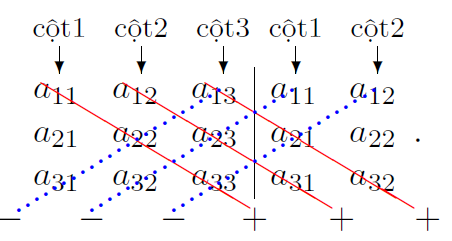
\includegraphics[scale=0.8]{C2_1}
\end{center}
\end{figure}
$$\left| A \right| = {a_{11}}{a_{22}}{a_{33}} + {a_{12}}{a_{23}}{a_{31}} + {a_{13}}{a_{21}}{a_{32}} - \left( {{a_{13}}{a_{22}}{a_{31}} + {a_{11}}{a_{23}}{a_{32}} + {a_{12}}{a_{21}}{a_{33}}} \right).$$
(Tổng ba đường chéo \textbf{đỏ} - tổng ba đường chéo \textbf{xanh})
\subsection{Khai triển định thức theo dòng và cột}
Cho $A = \left( {a_{ij}} \right) \in M_n \left( {\mathbb{R}} \right).$  Với mỗi $i,j \in \overline {1,n} ,$ ta gọi
$${c_{ij}} = {\left( { - 1} \right)^{i + j}}\left| {A\left( {\left. i \right|j} \right)} \right|$$
là \textit{phần bù đại số} của $a_{ij}.$
\begin{mybox}
\begin{theorem}
Cho $A = \left( {a_{ij}} \right) \in M_n \left( {\mathbb{R}} \right).$ Với mỗi $i,j \in \overline {1,n} ,$ ta gọi $c_{ij}$ là \textit{phần bù đại số} của $a_{ij}.$ Ta có công thức khai triển $\left| a \right|,$
\begin{itemize}
\item theo dòng $i:$ $\left| A \right| = \sum\limits_{k = 1}^n {{a_{ik}}{c_{ik}}} .$
\item theo dòng $j:$ $\left| A \right| = \sum\limits_{k = 1}^n {{a_{kj}}{c_{kj}}} .$
\end{itemize}
\end{theorem}
\end{mybox}
\begin{mybox}
\textbf{Nhận xét.} 
\[A\mathop  = \limits^{\text{ dòng }i} \sum\limits_{k = 1}^n {{a_{ik}}{{\left( { - 1} \right)}^{i + k}}\left| {A\left( {\left. i \right|k} \right)} \right|} \]
\[\begin{array}{*{20}{c}}
  {}&{\mathop  = \limits^{\text{cột } j} } 
\end{array}\sum\limits_{k = 1}^n {{a_{kj}}{{\left( { - 1} \right)}^{k + j}}\left| {A\left( {\left. k \right|j} \right)} \right|} \]
\end{mybox}
\begin{mybox}
\textbf{Lưu ý.} Khi tính định thức của ma trận ta nên chọn dòng hay cột có nhiều số $0$ để khai triển.
\end{mybox}
\begin{mybox}
\textbf{Mệnh đề.} Cho $A  \in M_n \left( {\mathbb{R}} \right).$ Khi đó:
\begin{itemize}
\item $\left| {{A^{\mathrm{T}}}} \right| = \left| A \right|.$
\item Nếu $A$ có một dòng hay một cột bằng không thì $\left| A \right| = 0.$
\item Nếu $A$ là ma trận tam giác thì $\left| A \right|$ được tính bằng tích các phần tử trên đường chéo, nghĩa là
$$\left| A \right| = a_{11} \times a_{22} \times ... \times a_{nn}.$$
\end{itemize}
\end{mybox}
\begin{mybox}
\begin{theorem}
Nếu $A, B  \in M_n \left( {\mathbb{R}} \right)$ thì $\left| {AB} \right| = \left| A \right|\left| B \right|.$
\end{theorem}
\end{mybox}
\textbf{Hệ quả.} Cho $A, A_1, A_2, ..., A_m  \in M_n \left( {\mathbb{R}} \right)$ và $k \in {\mathbb{N}^ * }.$ Khi đó
\begin{itemize}
\item $\left| {{A_1}{A_2}...{A_m}} \right| = \left| {{A_1}} \right|\left| {{A_2}} \right|...\left| {{A_n}} \right|;$
\item $\left| {{A^k}} \right| = {\left| A \right|^k}.$
\end{itemize}
\begin{mybox}
\begin{theorem}
Cho $A, A'  \in M_n \left( {\mathbb{R}} \right).$ Khi đó
\begin{itemize}
\item Nếu $A\mathop  \to \limits_{i \ne j}^{{d_i} \leftrightarrow {d_j}} A'$ thì $\left| {A'} \right| =  - \left| A \right|;$
\item Nếu $A\mathop  \to \limits^{\alpha {d_i}} A'$ thì $\left| {A'} \right| = \alpha \left| A \right|$ hay $\left| A \right| = \frac{1}{\alpha }\left| {A'} \right|;$
\item Nếu $A\mathop  \to \limits_{i \ne j}^{{d_i} + \beta {d_j}} A'$ thì $\left| {A'} \right| = \left| A \right|.$
\end{itemize}
\end{theorem}
\end{mybox}
\textbf{Hệ quả.} Cho $A  \in M_n \left( {\mathbb{R}} \right).$ Khi đó, với mọi $\alpha \in \mathbb{R},$ ta có
$$\left| {\alpha A} \right| = {\alpha ^n}\left| A \right|.$$
\begin{mybox}
\textbf{Lưu ý.} Vì $\left| {{A^{\mathrm{T}}}} \right| = \left| A \right|$ nên trong quá trình tính định thức ta có thể sử dụng các phép biến đổi sơ cấp trên cột. 
\end{mybox}
\begin{mybox}
\textbf{Lưu ý.} Trong quá trình tính định thức, phép biến đổi sơ cấp loại 3 được khuyến khích dùng bởi vì nó không làm thay đổi giá trị định thức.
\end{mybox}
\section{Định thức và ma trận khả nghịch}
\subsection{Ma trận phụ hợp}
Cho $A = \left( {a_{ij}} \right) \in M_n \left( {\mathbb{R}} \right).$ Đặt $C = \left( {c_{ij}} \right)$ với
$${c_{ij}} = {\left( { - 1} \right)^{i + j}}\left| {A\left( {\left. i \right|j} \right)} \right|$$
là phần bù đại số của $a_{ij}.$ Ta gọi ma trận chuyển vị $C^{\mathrm{T}}$ của $C$ là \textit{ma trận phụ hợp} (hay \textit{ma trận phó}) của $A,$ ký hiệu là $\mathrm{adj} \left( A \right).$
\subsection{Nhận diện ma trận khả nghịch}
\begin{mybox}
\begin{theorem}
Ma trận vuông $A$ khả nghịch khi và chỉ khi $\left| A \right| \ne 0.$ Hơn nữa
$${A^{ - 1}} = \frac{1}{{\left| A \right|}}\mathrm{adj}\left( A \right).$$
\end{theorem}
\end{mybox}
\textbf{Hệ quả.} Ma trận $A = \left( {\begin{array}{*{20}{c}}
  a&b \\ 
  c&d 
\end{array}} \right)$ khả nghịch khi và chỉ khi $ad - bc \ne 0.$ Khi đó
$${A^{ - 1}} = \frac{1}{{ad - bc}}\left( {\begin{array}{*{20}{c}}
  d&{ - b} \\ 
  { - c}&a 
\end{array}} \right).$$
\begin{mybox}
\textbf{Mệnh đề.} Cho $A  \in M_n \left( {\mathbb{R}} \right)$ và $A$ khả nghịch. Khi đó
\begin{itemize}
\item $\left| {{A^{ - 1}}} \right| = \frac{1}{{\left| A \right|}};$
\item $\left| {\mathrm{adj}\left( A \right)} \right| = {\left| A \right|^{n - 1}}.$
\end{itemize}
\end{mybox}
\section{Ứng dụng định thức để giải hệ phương trình tuyến tính}
\subsection{Quy tắc Cramer}
\begin{mybox}
\begin{theorem}
Cho hệ phương trình tuyến tính $AX = B$ gồm $n$ ẩn và $m$ phương trình (ma trận $A$ có $m$ dòng và $n$ cột). Đặt
$$\Delta  = \det \left( A \right);\begin{array}{*{20}{c}}
  {}&{}&{{\Delta _i}} 
\end{array} = \det \left( {{A_i}} \right),\forall i \in \overline {1,n} ,$$
trong đó $A_i$ là ,a trận có từ $A$ bằng cách thay cột $i$ bằng cột $B.$ Khi đó
\begin{itemize}
\item Nếu $\Delta \ne 0$ thì hệ có một nghiệm duy nhất là
$${x_i} = \frac{{{\Delta _i}}}{\Delta },\forall i \in \overline {1,n} .$$
\item Nếu $\Delta = 0$ và $\Delta_i \ne 0$ với một $i$ nào đó thì hệ vô nghiệm.
\item $\Delta = 0$ và $\Delta_i = 0$ $\forall i \in \overline {1,n} $ thì hệ vô nghiệm hoặc vô số nghiệm. Trong trường hợp này ta phải dùng phương pháp Gauss hoặc Gauss $-$ Jordan để giải.
\end{itemize}
\end{theorem}
\end{mybox}
\subsection{Giải và biện luận hệ phương trình tuyến tính bằng Cramer}
\chapter{Cấu trúc electron trong nguyên tử}
\section{Một số khám phá vật lý quan trọng đầu thế kỷ XX}
\subsection{Sóng điện từ}
Bốn đặc trưng cơ bản của sóng điện từ:
\begin{itemize}
\item Tốc độ truyền sóng $C$,
\item Bước sóng $\lambda,$
\item Tần số $\nu,$
\item Cường độ.
\end{itemize}
$$C = \lambda \cdot \nu.$$
Hiện tượng giao thoa ánh sáng và hiện tượng nhiễu xạ tia X là bằng chứng cho thấy bản chất sóng của sóng điện từ.
\subsection{Quang phổ}
\subsubsection{Quang phổ ánh sáng khả kiến}
Hiện tượng tán sắc ánh sáng: khi chiếu ánh sáng mặt trời qua lăng kính, tia sáng đỏ bị lệch hướng ít nhất, tia sáng tím bị lệch hướng nhiều nhất.\\
Quang phổ của ánh sáng khả kiến là quang phổ liên tục.
\subsubsection{Quang phổ nguyên tử}
Khi cho dòng điện phóng qua các ống chứa khí hay hơi nguyên tử, thu được bức xạ có bước sóng rời rạc.
\begin{itemize}
\item Mỗi loại khí có phổ vạch đặc trưng khác nhau, giống như mỗi người có dấu vân tay khác nhau.
\item Quang phổ này do nguyên tử phát ra nên gọi là phổ nguyên tử, hay phổ phát xạ nguyên tử, hay phổ vạch.
\end{itemize}
\subsubsection{Quang phổ phát ra từ các vật nóng}
\begin{itemize}
\item Khi đốt nóng, các vật rắn phát ra bức xạ với bước sóng liên tục.
\item Khi tăng nhiệt độ, bước sóng với cường độ cực địa di chuyển về phía sóng ngắn hơn.
\end{itemize}
\subsection{Khái niệm lượng tử ánh sáng của Max Planck}
Năng lượng có tính gián đoạn tương tự như vật chất.\\
Năng lượng lượng tử của sóng điện từ;
$$E = h \nu,$$ trong đó:
\begin{itemize}
\item $\nu:$ là tần số ánh sáng,
\item $h:$ là hằng số Planck, có giá trị là $6.626 \cdot 10^{- 34} \mathrm{Js}.$
\end{itemize}
\subsection{Hiện tượng quang điện và thuyết lưỡng nguyên ánh sáng của Albert Einstein}
\subsubsection{Hiện tượng quang điện}
Kết quả thí nghiệm cho thấy:
\begin{itemize}
\item Khi $\nu > \nu_0$ thì mới có sự thoát ra của electron, gọi là tần số ngưỡng quang điện.
\item Cường độ dòng quang điện tăng theo cường độ ánh sáng chiếu vào.
\item Động năng của electron tăng theo tần số $\nu$ của ánh sáng chiếu vào.
\item Mỗi kim loại có tần số ngưỡng quang điện $\nu_0$ khác nhau.
\end{itemize}
\subsubsection{Thuyết lưỡng nguyên ánh sáng của Einstein}
\begin{itemize}
\item Bức xạ điện từ không chỉ có tính sóng mà còn có tính hạt.
\item Bức xạ điện từ là dòng các photon, mỗi photon có năng lượng nhất định $E = h \nu.$
\item Những photon có $\nu > \nu_0$ thì electron mới tách khỏi nguyên tử.
\item Khi cường độ photon tăng thì số lượng các photon càng nhiều, số lượng electron bật ra khỏi bề mặt kim loại càng nhiều, cường độ dòng quang điện càng lớn.
\item Động năng của electron được tính như sau:
$$E_{d} = \frac{1}{2}mv^2 = E - E_0 = h \nu - h \nu_0.$$
\item Photon không có khối lượng nghỉ, nhưng có khối lượng khi di chuyển. Năng lượng của photon được tính theo công thức:
$$E = mc^2.$$
\item Khi chiếu chùm photon vào chùm electron, khi có va chạm photon chuyển một phần năng lượng cho electron. Như vậy, ánh sáng có tính lưỡng nguyên: sóng hạt.
\end{itemize}
\section{Mô hình nguyên tử $\mathrm{H}$ của Bohr}
\subsection{Mô hình nguyên tử $\mathrm{H}$ của Bohr}
Năm 1923, Niels Bohr kết hợp vật lý cổ điển với khái niệm lượng tử của Planck để đưa ra mô hình nguyên tử của $\mathrm{H}.$
\begin{itemize}
\item Electron chỉ được phép chuyển động trên một số quỹ đạo nhất định, gọi là \textbf{quỹ đạo dừng.}
\item Khi ở một trạng thái dừng nào đó, electron có năng lượng xác định. Electron trên quỹ đạo dừng chỉ mang moment góc:
$$m \nu r = \frac{nh}{2 \pi}.$$
\item Nguyên tử chỉ háp thu hay phát xạ năng lượng khi electron di chuyển từ quỹ đạo dừng này sang quỹ đạo dừng khác. Năng lượng hấp thu hay phát xạ khi đó là:
$$\Delta E = E_{\text{trạng thái cuối}} - E_{\text{trạng thái đầu}}.$$
\end{itemize}
\subsection{Nhược điểm của mô hình nguyên tử $\mathrm{H}$ của Bohr}
\begin{itemize}
\item Kết quả không đúng với các nguyên tử khác.
\item Mô hình Bohr là sự kết hợp thô sơ giữa các định luật vật lý cổ điển và không cổ điển mà không dựa trên cơ sở khoa học.
\end{itemize}
\section{Những luận điểm cơ sở và những ý tưởng chính dẫn đến thuyết cơ học lượng tử}
\subsection{Giả thiết của Louis de Broglie $-$ Tính lưỡng nguyên của vật chất}
Nếu ánh sáng có cả tính sóng và hạt thì vật chất, đặc biệt là các hạt nhỏ, cũng có thể có đồng thời hai tính hạt và sóng.
$$\lambda = \frac{h}{mv},$$
trong đó:
\begin{itemize}
\item $h:$ hằng số Planck,
\item $m:$ khối lượng của vật,
\item $v:$ vận tốc di chuyển của vật.
\end{itemize}
Hiện tượng nhiễu xạ electron chứng tỏ vật chất $-$ hay ít nhất là electron $-$ có tính sóng.\\
Năng lượng vừa có tính sóng vừa có tính hạt; vật chất có tính hạt, cũng có tính sóng.
\subsection{Nguyên lý bất định Heisenberg}
Không thể xác định chính xác đồng thời tốc độ và vị trí của electron.
$$\Delta x \times \Delta p \geqslant \frac{h}{4 \pi}.$$
Thế giới vi hạt tuân theo nguyên lý bất định Heisenberg vì chúng có cả hai đặc tính sóng và hạt.
\subsection{Phương trình sóng Schrodinger mô tả chuyển động của electron trong nguyên tử hydrogen}
Phương trình sóng Schrodinger cho nguyên tử $\mathrm{H}$ có một nhân mang điện tích dương và một electrong mang điện tích âm có dạng sau:
$$\frac{{{\mathrm{d}^2}\Psi }}{{\mathrm{d}{x^2}}} = \left( {\frac{{2\pi }}{\lambda }} \right)\Psi .$$
\section{Mô hình nguyên tử hydrogen theo thuyết cơ học lượng tử}
\subsection{Kết quả giải phương trình Schrodinger cho nguyên tử hydrogen: ba số lượng tử, hàm sóng $\Psi$, và orbital nguyên tử}
Giải phương trình Schrodinger cho nguyên tử hydrogen dẫn đến các hàm sóng $\Psi$ với ba tham số $n, \ell, m_{\ell},$ gọi là ba số lượng tử, đặc trưng cho các hàm sóng:
\begin{itemize}
\item $n$ gọi là \textbf{số lượng tử chính,} nhận giá trị là các số tự nhiên dương $1, 2, 3, ...$
\item $\ell$ là \textbf{số lượng tử moment góc,} còn gọi là \textbf{số lượng tử phụ,} có các giá trị từ $0$ đến $n - 1.$
\item $m_{\ell}$ là \textbf{số lượng tử từ,} có giá trị từ $- \ell \to \ell.$
\end{itemize}
\subsection{Ý nghĩa của $\Psi$ $-$ orbital nguyên tử}
Ý nghĩa của hàm $\Psi:$
\begin{itemize}
\item Phương trình $\Psi$ mô tả chuyển động của electron trong nguyên tử.
\item $\Psi ^2$ đặc trưng cho xác suất bắt gặp electron (chính xác hơn là mật độ electron) tại vị trí nào đó quanh nhân nguyên tử.
\item Vùng không gian quanh nhân có khả năng tìm thấy điện tử nhiều nhatasm gọi là orbital nguyên tử (Atomic Orbital, AO), hay đám mây điện tử, vân đạo điện tử.
\item Bộ ba số lượng tử $n, \ell, m_{\ell}$ đặc trưng cho mỗi AO tương ứng. 
\end{itemize}
Số lượng tử chính $n:$
\begin{itemize}
\item Đặc trưng cho \textbf{kích thước và năng lượng} của orbital.
\item Các orbital có năng lượng bằng nhau gọi là \textbf{orbital suy biến năng lượng.}
\end{itemize}
Số lượng tử phụ $\ell:$
\begin{itemize}
\item Đặc trưng cho \textbf{moment động lượng của electron} và \textbf{hình dạng của orbital.}
\item Hình dạng của orbital được quy ước là hình dạng của vùng không gian có xác suất bắt gặp electron cao nhất.
\item Các orbital có $\ell = 0$ ($s$) có dạng hình cầu, các orbital có $\ell = 1$ ($p$) có dạng hình số tám nổi, các orbital có $\ell = 2$ ($d$) có hình dạng phức tạp hơn.
\end{itemize}
Số lượng tử phụ $m_{\ell}:$
\begin{itemize}
\item Đặc trưng cho \textbf{sự định hướng các orbital trong không gian.}
\end{itemize}
\subsection{Spin của electron $-$ số lượng tử thứ tư}
Bản thân các electron có moment từ nội tại, có thể định hướng theo hai kiểu khác nhau dưới tác dụng của từ trường ngoài, gọi là \textit{spin} của electron. \\
Do đó, ngoài ba số lượng tử xuất phát từ phương trình Schrodinger, cần có số lượng tử thứ tư biểu diễn cho đặc tính từ của electron, gọi là \textit{số lượng tử spin,} ký hiệu là $m_s.$
\subsection{Nguyên tử nhiều electron}
\begin{itemize}
\item Tương tác của electron trong nguyên tử nhiều electron rất phức tạp.
\item Không thể viết và giải phương trình Schrodinger một cách chính xác cho nguyên tử nhiều electron.
\item Chỉ có thể thiết lập và giải gần đúng phương trình Schrodinger cho nguyên tử nhiều electron bằng nhiều phương pháp khác nhau.
\end{itemize}
Các electron trên orbital $ns$ có mật độ electron gần nhân cao hơn electron trên orbital $np$ và $nd$ cùng lớp.
\subsection{Nguyên lý loại trừ Pauli $-$ Quy tắc Hund $-$ Quy tắc Klechkowski}
\subsubsection{Nguyên lý loại trừ Pauli}
Mỗi orbital nguyên tử chỉ có thể chứa tối đa hai electron với spin khác nhau. Để phân biệt hai electron này, ta dùng số lượng tử spin $m_s.$\\
Trong một nguyên tử \textbf{không thể có hai electron có cùng bốn số lượng tử.}
\subsubsection{Quy tắc Hund}
Các electron có khuynh hướng phân bố đều vào các orbital sao cho \textbf{tổng spin của các electron trong nguyên tử là cực đạ}i để tương tác đẩy giữa các electron trong cùng phân lớp là thấp nhất.
\subsubsection{Quy tắc Klechkowski}
Là quy tắc để ghi nhớ việc điền electron.
\chapter{Ánh xạ tuyến tính}
\section{Định nghĩa}
\subsection{Ánh xạ}
Một \textit{ánh xạ} $f$ từ tập $X$ vào tập $Y$ là một phép liên kết từ $X$ vào $Y$ sao cho mỗi phần tử $x$ của $X$ được liên kết duy nhất một phần tử $y$ của $Y,$ ký hiệu $y = f \left( x \right).$
$$\begin{gathered}
  f:\begin{array}{*{20}{c}}
  {}&{X \to Y} 
\end{array} \hfill \\
  \begin{array}{*{20}{c}}
  {}&{}&{x \mapsto y = f\left( x \right)} 
\end{array}. \hfill \\ 
\end{gathered} $$
Khi đó $X$ được gọi là \textit{tập nguồn,} $Y$ được gọi là \textit{tập đích.}
\subsection{Ánh xạ tuyến tính}
Cho $V$ và $W$ là hai không gian vector trên $\mathbb{R}.$ Ta nói ánh xạ $f: V \to W$ là một \textit{ánh xạ tuyến tính} nếu thỏa hai điều kiện sau:
\begin{itemize}
\item $f \left( {u + v} \right) = f \left( u \right) + f \left( v \right)$ với mọi $u, v \in V;$
\item $f \left( {\alpha u} \right) = \alpha f \left( u \right)$ với mọi $\alpha \in \mathbb{R}$ và với mọi $u \in V.$
\end{itemize}
\textbf{Nhận xét.} Hai điều kiện trong định nghĩa trên có thể được thay thế bằng một điều kiện:
$$f \left( {\alpha u + v} \right) = \alpha f \left( u \right) + f \left( v \right), \forall \alpha \in \mathbb{R}, \forall u, v \in V.$$
Ký hiệu:
\begin{itemize}
\item $\mathbf{L \left( {V, W} \right)}$ là tập hợp các ánh xạ tuyến tính từ $V$ vào $W.$
\item Nếu $f \in L \left( {V, V} \right)$ thì $f$ được gọi là một \textit{toán tử tuyến tính} trên $V.$ Viết tắt $f \in L \left( V \right).$
\end{itemize}
\begin{mybox}
\textbf{Mệnh đề.} Cho $f: V \to W$ là ánh xạ tuyến tính. Khi đó
\begin{itemize}
\item $f \left( 0 \right) = 0;$
\item Với mọi $u \in V,$ ta có $f \left( {- u} \right) = - f \left( u \right);$
\item Với mọi $u_1, u_2, ..., u_m \in V$ và với mọi $\alpha_1, \alpha_2, ..., \alpha_m \in \mathbb{R},$ ta có
$$f\left( {{\alpha _1}{u_1} + {\alpha _2}{u_2} + ... + {\alpha _m}{u_m}} \right) = {\alpha _1}f\left( {{u_1}} \right) + {\alpha _2}f\left( {{u_2}} \right) + ... + {\alpha _m}f\left( {{u_m}} \right).$$
\end{itemize}
\end{mybox}
\begin{mybox}
\begin{theorem}
Cho $V$ và $W$ là hai không gian vector và $\mathbf{B} = \left\{ {u_1, u_2, ..., u_n} \right\}$ là cơ sở của $V.$ Khi đó, nếu $S = \left\{ {v_1, v_2, ..., v_n} \right\}$ là một tập con của $W$ thì \textit{tồn tại duy nhất} một ánh xạ tuyến tính $f: V \to W$ sao cho
$$f\left( {{u_1}} \right) = {v_1},f\left( {{u_2}} \right) = {v_2},...,f\left( {{u_n}} \right) = {v_n}.$$
Hơn nữa, nếu ${\left[ u \right]_{\mathbf{B}}} = \left( \begin{gathered}
  {\alpha _1} \hfill \\
  {\alpha _2} \hfill \\
  ... \hfill \\
  {\alpha _n} \hfill \\ 
\end{gathered}  \right)$ thì 
$$f\left( u \right) = {\alpha _1}f\left( {{u_1}} \right) + {\alpha _2}f\left( {{u_2}} \right) + ... + {\alpha _n}f\left( {{u_n}} \right).$$
\end{theorem}
\end{mybox}
\section{Nhân và ảnh của ánh xạ tuyến tính}
\subsection{Không gian nhân}
Cho $f: V \to W$ là một ánh xạ tuyến tính. Ta đặt
$$\ker f = \left\{ {u \in \left. V \right|f\left( u \right) = 0} \right\}$$
Khi đó $\ker f$ là không gian con của $V,$ ta gọi $\ker f$ alaf \textit{không gian nhân} của $f.$
\begin{mybox}
\textbf{Nhận xét.} Dựa vào định nghĩa, ta được
$$u \in \ker f \Leftrightarrow f \left( u \right) = 0.$$
\end{mybox}
\subsection{Không gian ảnh}
Cho $f: V \in W$ là một ánh xạ tuyến tính. Ta đặt
$$\operatorname{Im} f = \left\{ {\left. {f\left( u \right)} \right|u \in V} \right\}.$$
Khi đó $\operatorname{Im} f$ là không gian con của $W,$ ta gọi $\operatorname{Im} f$ là \textit{không gian ảnh} của $f.$
\begin{mybox}
\begin{theorem}
Cho $f: V \in W$ là một ánh xạ tuyến tính. Khi đó, nếu
$$S = \left\{ {{u_1},{u_2},...,{u_m}} \right\}$$ 
là tập sinh của $V$ thì
$$f\left( S \right) = \left\{ {f\left( {{u_1}} \right),f\left( {{u_2}} \right),...,f\left( {{u_m}} \right)} \right\}$$
là tập sinh của $\operatorname{Im} f.$
\end{theorem}
\end{mybox}
\begin{mybox}
\textbf{Nhận xét.} Dựa vào định lí trên, để tìm cơ sở của $\operatorname{Im} f,$ ta chọn một tập sinh $S$ của $V$ (để đơn giản ta nên chọn cơ sở chính tắc). Khi đó $\operatorname{Im} f$ sinh bởi tập ảnh của $S.$
\end{mybox}
\begin{mybox}
\begin{theorem}
Cho $f: V \in W$ là một ánh xạ tuyến tính và $V$ hữu hạn chiều. Khi đó
$$\dim \operatorname{Im} f + \dim \ker f = \dim V.$$
\end{theorem}
\end{mybox}
\section{Ma trận biểu diễn ánh xạ tuyến tính}
Cho $\mathbf{B} = \left( {u_1, u_2, ..., u_n} \right)$ là cơ sở của $V,$  
$\mathbf{C} = \left( {v_1, v_2, ..., v_m} \right)$ là cơ sở của $W$ và $f \in L \left( {V, W} \right).$ Ta đặt
$$P = \left( {{{\left[ {f\left( {{u_1}} \right)} \right]}_{\mathbf{C}}}{{\left[ {f\left( {{u_2}} \right)} \right]}_{\mathbf{C}}}...{{\left[ {f\left( {{u_n}} \right)} \right]}_{\mathbf{C}}}} \right).$$
Khi đó ma trận $P$ được gọi là \textit{ma trận biểu diễn} của ánh xạ $f$ theo cặp cơ sở $\mathbf{B}, \mathbf{C},$ ký hiệu là $P = {\left[ f \right]_{\mathbf{B},\mathbf{C}}}$ (hoặc $\left[ f \right]_{\mathbf{B}}^{\mathbf{C}}$).
\begin{mybox}
\textbf{Nhận xét.} Khi $V = \mathbb{R}^n, W = \mathbb{R}^m,$ ta có phương pháp tìm $P = {\left[ f \right]_{\mathbf{B},\mathbf{C}}}$ như sau:
\begin{itemize}
\item Tính $f\left( {{u_1}} \right),f\left( {{u_2}} \right),...,f\left( {{u_n}} \right).$
\item Đặt $M = \left( {\begin{array}{*{20}{c}}
  {v_1^{\mathrm{T}}}&{v_2^{\mathrm{T}}}&{...}&{\left. {v_m^{\mathrm{T}}} \right|\begin{array}{*{20}{c}}
  {f{{\left( {{u_1}} \right)}^{\mathrm{T}}}}&{f{{\left( {{u_2}} \right)}^{\mathrm{T}}}}&{...}&{f{{\left( {{u_n}} \right)}^{\mathrm{T}}}} 
\end{array}} 
\end{array}} \right).$
\item Dùng thuật toán Gauss $-$ Jordan, đưa $M$ về dạng $\left( {\left. {{I_m}} \right|P} \right).$
\item Khi đó $\left[ f \right]_{\mathbf{B},\mathbf{C}} = P.$
\end{itemize}
\end{mybox}
Cho $\mathbf{B} = \left( {u_1, u_2, ..., u_n} \right)$ là cơ sở của $V$ và $f \in L \left( V \right).$ Khi đó ma trận $\left[ f \right]_{\mathbf{B},\mathbf{B}}$ được gọi là \textit{ma trận biểu diễn toán tử tuyến tính $f,$} ký hiệu là $\left[ f \right]_{\mathbf{B}}.$ Rõ ràng
$$\left[ f \right]_{\mathbf{B}} = \left( {{{\left[ {f\left( {{u_1}} \right)} \right]}_{\mathbf{B}}}{{\left[ {f\left( {{u_2}} \right)} \right]}_{\mathbf{B}}}...{{\left[ {f\left( {{u_n}} \right)} \right]}_{\mathbf{B}}}} \right).$$
\begin{mybox}
\begin{theorem}
Cho $V$ và $W$ là các không gian vector; $\mathbf{B}, \mathbf{B'}$ và $\mathbf{C}, \mathbf{C'}$ tương ứng là các cặp cơ sở của $V$ và $W.$ Khi đó, với mọi ánh xạ tuyến tính $f: V \to W$ ta có
\begin{itemize}
\item $\forall u \in V,{\left[ {f\left( u \right)} \right]_{\mathbf{C}}} = {\left[ f \right]_{\mathbf{B},\mathbf{C}}}{\left[ u \right]_{\mathbf{B}}}.$
\item ${\left[ f \right]_{\mathbf{B'},\mathbf{C'}}} = {\left( {\mathbf{C} \to \mathbf{C'}} \right)^{ - 1}}{\left[ f \right]_{\mathbf{B},\mathbf{C}}}\left( {\mathbf{B} \to \mathbf{B'}} \right).$
\end{itemize}
\end{theorem}
\end{mybox}
\textbf{Hệ quả.} Cho $\mathbf{B}$ và $\mathbf{B'}$ là hai cơ sở của không gian hữu hạn chiều $V.$ Khi đó đối với mọi toán tử tuyến tính $f \in L \left( V \right)$ ta có
\begin{itemize}
\item $\forall u \in V,{\left[ {f\left( u \right)} \right]_{\mathbf{B}}} = {\left[ f \right]_{\mathbf{B}}}{\left[ u \right]_{\mathbf{B}}}.$
\item ${\left[ f \right]_{\mathbf{B'}}} = \left(\mathbf{B}  \to \mathbf{B'} \right)^{-1}{\left[ f \right]_{\mathbf{B}}}\left(\mathbf{B}  \to \mathbf{B'} \right).$
\end{itemize}
\end{document}